\documentclass{article}
\usepackage{tikz}
\usetikzlibrary{graphs}
\usetikzlibrary{graphs.standard}

\begin{document}

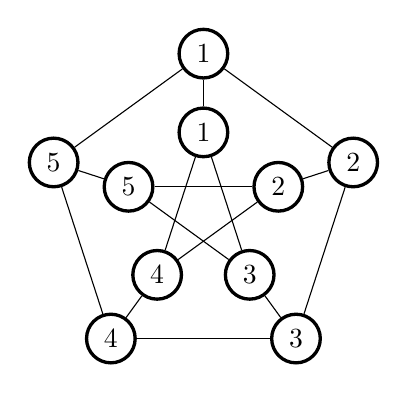
\begin{tikzpicture}[every node/.style={draw,circle,very thick}]
\graph[clockwise, radius=2cm] {subgraph C_n [n=5,name=A] };
\graph[clockwise, radius=1cm, n=5, name=B] { subgraph I_n };

\foreach \i [evaluate={\j=int(mod(\i+2+4,5)+1)}]
in {1,2,3,4,5}{
	\draw (A \i) -- (B \i);
	\draw (B \j) -- (B \i);
}
\end{tikzpicture}

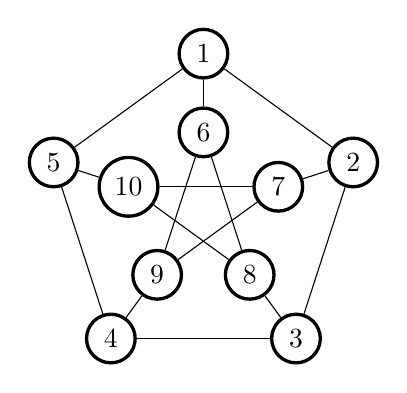
\begin{tikzpicture}[every node/.style={draw,circle,very thick}]
\graph[clockwise, radius=2cm, n=5,name=A] {subgraph C_n };
\graph[clockwise, radius=1cm, n=5, name=B] { 1/"6", 2/"7", 3/"8", 4/"9", 5/"10"; subgraph I_n };

\foreach \i [evaluate={\j=int(mod(\i+2+4,5)+1)}]
in {1,2,3,4,5}{
	\draw (A \i) -- (B \i);
	\draw (B \j) -- (B \i);
}
\end{tikzpicture}

\end{document}